\chapter{Analýza}
\section{Funkční speficikace}
Framework musí umožňovat uživateli vytvářet a dále pracovat s vytvořenými komponentami. Komponenty budou procházet určitým životním cyklem. Kromě samotných komponent musí framework poskytovat i dodatečné funkcionality, které jsou spojeny se získáváním dat, jejich propagací na klienta, zabezpečení, organizací komponent, lokalizací a skinováním komponent.
\subsection{Funkční požadavky}
Z dosavadního popisu problému byly vytvořeny následující požadavky na systém.
\begin{itemize}
\item Framework bude umožňovat generovat metadata objektů, na základě kterých budou generovány komponenty.
\item Framework bude umožňovat vygenerovat formulář nebo tabulku na základě dat získaných ze serveru.
\item Framework bude umožňovat získat data ze serveru.
\item Framework bude umožňovat naplnit formulář i tabulku daty.
\item Framework bude umožňovat odeslat data z formuláře zpět na server.
\item Framework bude umožňovat používat lokalizační resource bundly.
\item Framework bude umožňovat validaci dat na základě metadat, která obdržel od serveru.
\item Framework bude umožňovat klientovi překrýt chybové validační hlášky.
\item Framework bude umožňovat skinovatelnost.
\item Framework bude umožňovat specifikovat zdroje ve formátu xml.
\item Framework bude umožňovat vytvářet vstupní pole, combo boxy, výstupní pole, textarea, checkboxy, option buttony.
\item Framework bude umožňovat vkládat do formulářových polí texty, čísla a datumy.
\item Framework bude umožňovat generování readonly komponent. 
\end{itemize} 
Z požadavků vyplívá, že framework bude umožňovat získání definici dat na serveru a poté je distribuuje koncovému uživateli. Koncový uživatel tedy nebude potřebovat znát obejkty, s kterými pracuje. Toto zaručí pružnou reakci na změnu dat a generování aktuálních formuláří či tabulek. 
\subsection{Nefunkční požadavky}
\begin{itemize}
\item Framework bude generovat části uživatelských rozhraní.
\item Framework bude nezávislý na platformě.
\end{itemize} 
\section{Popis architektury a komunikace}
Jak již bylo uvedeno, tak je definice objektů, na základě kterých se budou vytvářet komponenty, generována na serverové straně. Klient tedy komunikuje se serverem a vyžádá si tyto definice. Dále je potřeba definice na klientovi zpracovat. Definice budou platformově nezávislé. Budou tedy popisovat data v obecné formě, aby bylo možné generovat formuláře a tabulky nezávisle na platformě, jazyku a technologii. Referenční implementace bude napsána v jazyce Java pro Swingové aplikace. Data, která jsou zasílány ze serveru na klientovi by neměli ovlivňovat ostatní klienty, kteří framework nepoužívají.
\subsection{Metadata}
Metadata jsou data, která popisují jiná data. Framework, který je popsán v této práci generuje na serverové straně metadata a zasílá je na klienta, který na jejich základě sestaví komponenty a poté je schopný provádět nad daty operace. Klient musí být schopný zpětně sestavit data a odeslat je na server. Klient využívá klientskou část frameworku a server serverovou část. Z hlediska implementace je důležité, aby objekty nesoucí informace o metadatech byli stejné a bylo možné provést na klientovi generování na základě těchto dat.
Následující doménový model znázorňuje popis definic objektu, který je vytvořen po inspekci zadaného objektu. Inspekce vytvoří XML popis, který je převeden na obecný popis, jenž lze využít ke generování dat na klientovi. Tento obecný popis je zaslán klientovi, který využívá klientskou část frameworku. Klientská část frameworku očekává tyto objekty a na jejich základě je schopná vygenerovat uživatelské rozhraní. Na obrázku \ref{img:metadataModel} je zobrazen doménový model \cite{UmlArlow}, který je použit při popisu metadat objektu. Nejedná se o doménový model frameworku, ale pouze jeho části, která je zodpovědná za reprezentaci metadat. 

\begin{figure}[h!]
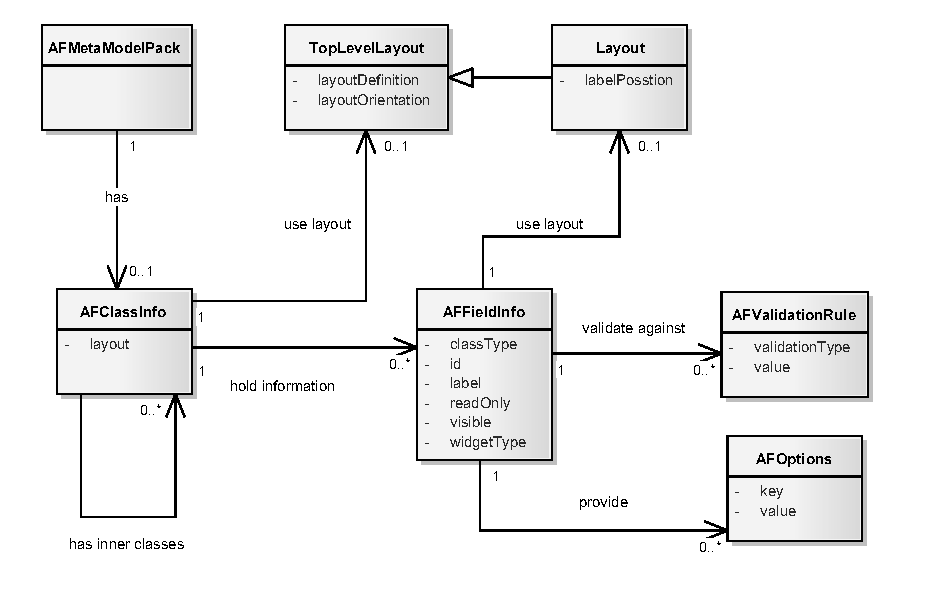
\includegraphics{images/domainModel}
\caption{Doménový model obejktů obsahující metadat o objektu, nad kterým byla provedena inspekce}
\label{img:metadataModel}
\end{figure}

\subsubsection{AFMetaModelPack}
Tato třída zapouzdřuje informace, které popisují objekt, nad kterým byla prováděna inspekce. Třída rovněž slouží jako fasáda a nabízí programátorovi upravení metadat po generování. V případě serveru je toto návratový typ zdroje, na který klient přistoupí chce li znát metadata, která zdroj poskytuje.
\subsubsection{AFClassInfo}
Tato třída udržuje informace o hlavním objektu, z kterého je vytvářena definice. Třída má dále reference na své vnitřní proměnné a své potomky. Na základě generování dat je potřeba udržet pořadí, v kterém byla nad jednotlivými komponenty prováděna inspekce. V případě inspekce dat je i reference na neprimitivní datový typ jeho proměnná. Nicméně je potřeba, aby klient byl schopný určit, že se jedná o složitý datový typ a určit jeho pořadí v aktuálním objektu, aby mohl rozhodnout na jaké pozici objekt zobrazit. 
\subsubsection{AFFieldInfo}
Tato třída je zodpovědná za poskytování detailních informací o proměnné objektu, nad kterým byla provedena inspekce. Třída udržuje název proměnné, widget, na který bude proměnná převedena, pravidla, která musí být splněna a název pod kterým, bude prezentována uživateli. Kromě těchto vlastností nese objekt také informace o tom, zdali je komponenta viditelná a zdali je pouze pro čtení.
\subsubsection{AFRule}
Každá proměnná má souhrn vlastností, které musí být splněny. Typ widgetu ještě vždy nemusí určovat datový typ komponenty. Dále neurčuje, zdali je pole povinné či nikoliv. Tento soubor vlastností je popisován v této třídě. Třída využívá ENUM, který specifikuje podporované validace. Důvodem je to, že klient musí být schopný vytvořit tyto validační pravidla a interpretovat je na komponentě svým vlastním způsobem, který je specifický pro technologii, kterou používá. Jednou z dalších výhod je validace XML, z kterého jsou pravidla vytvářena. Framework vytvoří pouze ty validační pravidla, která podporuje. Klient poté musí podporovaná pravidla interpretovat. 
\subsubsection{AFOptions}
Některé widgety umožňují, aby si uživatel vybral z několika předem připravených možností. Tyto možnosti musí být klientovi prezentovány. Tato třída udržuje informace o možnostech výběru v dané komponentě. Proměnná klíč je hodnota, která bude odeslána zpět na server a proměnná value je hodnota, která bude zobrazena klientovi. Tímto způsobem lze klientovi zobrazit jakýkoliv text, který bude zpětně mapován na jeho skutečnou hodnotu. Kromě textu lze samozřejmě zobrazit čísla či hodnoty výčtových typů.

\subsection{Server}
Server je zařízení či software, který umožňuje zpracovat požadavky od klientů a na jejich základě vytvořit odpověď. Server tedy poskytuje svým klientům určitý typ obsahu. Způsob a původ obsahu, který server poskytuje je pro klienta povětšinou neznámý. V současné době je velmi populární způsob, při kterém server získá data z vice zdrojů a poskytne je klientovi. Hovoříme o tzv mashup \cite{Tuchinda2008}. Mashup nemusí být pouze z veřejných zdrojů, lze využít i zdroje z privátních zdrojů, či lze k sestavení request využít další služby. Klient napojený na server tohoto typu nemusí mít o těchto dalších zdrojích vůbec žádnou povědomost a dotazuje se pouze vůči tomuto serveru, který zpracovává jeho požadavky. 
Klienti, kteří získávají data z veřejných, či privátních zdrojů serveru může být spousta. Mohou to být vlastní privátní aplikace, mobilní aplikace, javascriptoví klienti či další server, který pouze využívá veřejné zdroje serveru k sestavení odpovědi svým vlastním klientům. V těchto případech je potřeba zvážit způsob generování definic dat, které by mohly způsobit stávajícím klientům problémy. V ideálním případě, je tedy potřeba framework integrovat takovým způsobem aby byla zachována stávající funkcionalita a framework ji pouze rozšířil. 
Ke generování definic objektů jsou potřeba následující věci:
\begin{enumerate}
\item Objekt, jehož definice budou generovány.
\item Mapování, na základě, kterého bude rozhodnuto, o jaký typ komponenty půjde.
\item Definice komponenty včetně jejich vlastností jako jsou validace, layout a popis chování komponenty.
\item Layout, v kterém budou komponenty sestaveny.
\item Framework, který provede inspekci.
\item Framework, který bude inspekci řídit a bude interpretovat vygenerovaná data. Tento framework musí zároveň ověřit validitu jednotlivých komponent.
\end{enumerate}

Výše uvedené vlastnosti, nebudou mít vliv na změnu funkcionality. K inspekci a mapování bude využit framework AspectFaces \cite{aspectFaces}, který umožňuje na základě datových typů rozhodnout jakou komponentu využít. Definice komponent a jejich vlastností bude již v plné kompetenci vývojáře, nicméně základní komponenty a jejich chování bude předpřipraveno ve vzorovém projektu aby se vývojář mohl inspirovat.
Server využívá serverovou část.

\subsection{Klient}

\subsection{Případy užití}
Případy užití a jejich scénáře \cite{UmlArlow} specifikují chování systému. V této práci lze nahlížet na případy užití ze dvou stran. První z nich je koncový uživatel nebo-li vývojář, který framework využívá. Druhým z nich je samotný framework, který provádí akce, aby splnil úkol, který mu uživatel uložil. V této sekci se zaměříme na případy užití koncového uživatel, které specifikují použití frameworku. Na obrázku \ref{img:useCase} jsou zachyceny všechny tyto případy užití. Pro ukázku detailně rozebereme případ užítí na obrázku \ref{img:useCaseSmall}. Na tomto případu je znázorněno odeslání dat z vygenerovaného formuláře zpět na server. Součástí je samozřejmě validace zadaných dat a jejich zpětné sestavení, neboť formulář byl vytvořen na základě metadat a klient tedy zná pouze strukturu objektu popsanou těmito metadaty. 
\begin{figure}[h!]
\begin{center}
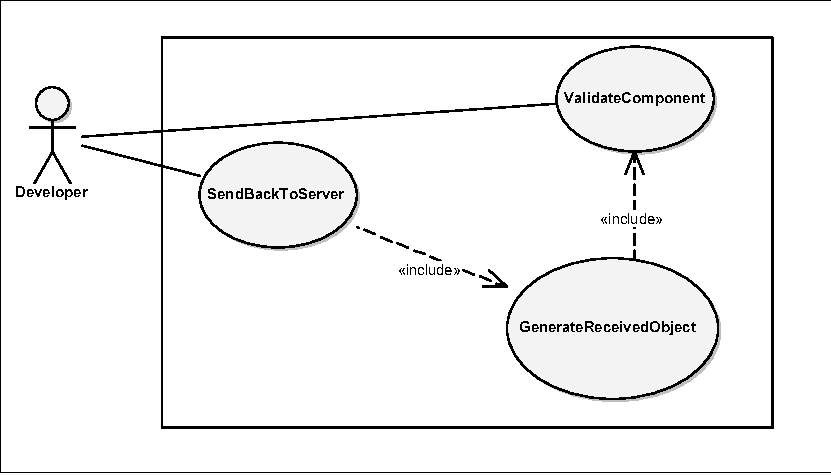
\includegraphics{images/useCaseSmall}
\caption{Část případů užití znázorňující odeslání dat na server z vygenerovaného formuláře}
\label{img:useCaseSmall}
\end{center}
\end{figure}
\subsubsection{Validace komponenty}
Tento případ užití je znázorněn na obrázku \ref{img:useCaseSmall} a jmenuje se ValidateComponent.

Případ užití: Validace komponenty\\
ID: 1\\
Popis: 
Uživatel využívá framework ke generování formulářů. Hlavním úkolem formuláře je možnost vkládat či upravovat data a odesílat je zpět na server. Před odesláním dat na server musí být provedena validace, aby se zajistilo, že bude formát dat serveru vyhovovat a bude umět s daty pracovat.
\\
Aktér: Uživatel\\
Vstupní podmínky:
\begin{enumerate}
\item Formulář musí být sestaven na základě metadat a framework musí znát formulář s kterým chce pracovat.
\end{enumerate}
Scénář:
\begin{enumerate}
\item Případ užití začíná obdržením požadavku od uživatele žadající validaci dat.
\item Systém vyhledá pole k validaci.
\item Dokud existují pole k validaci pak:
\begin{enumerate}
\item Systém získá konkrétní pole k validaci.
\item Systém určí typ komponenty a požádá builder, který ji sestavil o data.
\item Dokud existuje validace, která zatím nebylo na poli vykonána pak:
\begin{enumerate}
\item Systém požádá validátor o validaci.
\item Pokud validace selže pak:
\begin{enumerate}
\item Systém ukončí validování tohoto pole a zobrazí u něj chybovou validační hlášku.
\end{enumerate}
\end{enumerate}
\end{enumerate}
\end{enumerate}

Případ užití: Sestavení dat\\
ID: 2\\
Popis: 
Uživatel využívá framework ke generování formulářů. Hlavním úkolem formuláře je možnost vkládat či upravovat data a odesílat je zpět na server. Před odesláním dat na server musí být tyto data zpětně sestaveny, aby s nimi server dokázal pracovat.
\\
Aktér: Uživatel\\
Vstupní podmínky:
\begin{enumerate}
\item Formulář musí být sestaven na základě metadat a framework musí znát formulář s kterým chce pracovat. Framework musí znát formát dat, které server očekává.
\end{enumerate}
Scénář:
\begin{enumerate}
\item Případ užití začíná obdržením požadavku od uživatele žadající sestavení dat z formuláře.
\item Zahrnout(Validace komponenty).
\item Pokud validace dopadla úspěšně pak:
\begin{enumerate}
\item Systém získá pole, která budou odeslána.
\item Pokud exsituje pole, které ještě nebylo transformováno pak:
\begin{enumerate}
\item Systém určí typ komponenty a požádá builder, který ji sestavil o data.
\item Systém určí název proměnné a třídu, do které patří a nastaví ji data.
\end {enumerate}
\item Systém na základě formátu dat, které server očekává rozhodne v jakém formátu data zaslat a převede je na daný formát.
\end{enumerate}
\end{enumerate}

Výstupní podmínka:
\begin{enumerate}
\item Data ve formuláři byla převedena na objekt, s kterým umí server pracovat.
\end{enumerate}

Případ užití: Odeslání dat\\
ID: 3\\
Popis: 
Uživatel využívá framework ke generování formulářů. Hlavním úkolem formuláře je možnost vkládat či upravovat data a odesílat je zpět na server. Před odesláním dat na server musí být tyto data zpětně sestaveny, aby s nimi server dokázal pracovat a musí splnit validační kritería
\\
Aktér: Uživatel\\
Vstupní podmínky:
\begin{enumerate}
\item Formulář musí být sestaven na základě metadat a framework musí znát formulář s kterým chce pracovat. Framework musí znát zdroj, na který mají být data odeslána a všechny potřebné informace, které zdroj vyžaduje.
\end{enumerate}
Scénář:
\begin{enumerate}
\item Případ užití začíná obdržením požadavku od uživatele žadající odeslání formuláře na server.
\item Zahrnout(Validace komponenty).
\item Zahrnout(Sestavení dat)
\item Dokud je validace či sestavení dat neúspěšné pak:
\begin{enumerate}
\item Systém zobrazí chybové hlášky a určí, u kterých poli nastala chyba
\item Uživatel chybu opraví a požádá systém o opětovnou validaci a sestavení dat.
\end{enumerate}
\item Systém vytvoří připojení na specifikovaný zdroj a odešle data.
\item Pokud odeslání selhalo pak:
\begin{enumerate}
\item Systém zobrazí chybovou hlášku, že nebylo možné data odeslat včetně odpovědi od serveru, je-li nějaká.
\end{enumerate}
\end{enumerate}

Výstupní podmínka:
\begin{enumerate}
\item Data byla odeslána.
\end{enumerate}


\section{Omezení frameworku}
\section{Uživatelé a zabezpečení}